\documentclass[11pt]{article}

\usepackage[a4paper,margin=2cm,top=3cm]{geometry}

% graphics
\usepackage{tikz}
\usepackage{graphicx}

% math
\usepackage{amsmath}
\usepackage{amsfonts}

\usepackage[indentafter]{titlesec}

%listings
\usepackage{xcolor}
\usepackage{listings}
\lstset{
	backgroundcolor=\color{gray!10!white},   
	basicstyle=\footnotesize\ttfamily,
	breaklines=true,
	commentstyle=\color{gray},
	escapeinside={~}{~},
	frame=single,
	keywordstyle=\color{blue},
	language=C,
	numbers=left,
	numbersep=5pt,
	showstringspaces=false,   
	numberstyle=\tiny\color{gray},
	rulecolor=\color{gray},
	stringstyle=\color{purple},
	tabsize=4}
\lstnewenvironment{code}{\latin}{\endlatin}

% header
\usepackage{fancyhdr}
 
\fancyhf{}
\lhead{دانشگاه صنعتی شریف}
\rhead{تمرینِ علی ادیبی}
\chead{مبانی برنامه‌نویسی}
\cfoot{\thepage}
 

% others
\usepackage{tabularx}
\usepackage{array}
\usepackage{fixltx2e}

\usepackage[hidelinks]{hyperref}

% persian
\usepackage[extrafootnotefeatures]{xepersian}
\settextfont{IRZar}
\setlatintextfont[Scale=0.8]{Liberation Serif}
\setdigitfont{IRZar}

\begin{document}


%%% first page %%%
	\thispagestyle{empty}
	
	\begin{center}
		به نامِ خدا
	
		\vskip 60mm
	
		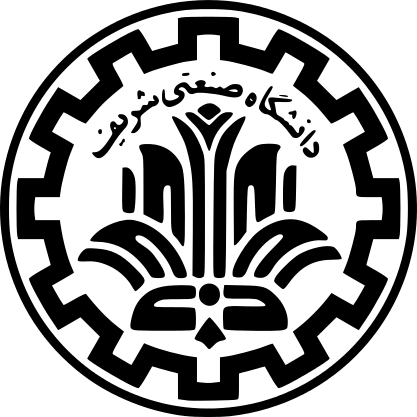
\includegraphics[width=4.5cm]{sharif-logo}\\
		\vskip 10mm
		\huge{درسِ مبانیِ برنامه‌سازی} \\
		\bigskip
		\bigskip
		\large{نیم‌سالِ اول ۹۷-۹۶} \\
		\bigskip
		دانشکدهٔ مهندسیِ کامپیوتر\\
		\medskip
		دانشگاهِ صنعتیِ شریف \\
		\bigskip
		\hrule height 2pt
		\medskip
		
		{\def\arraystretch{1.3}
		\begin{tabular}{>{\raggedright}p{0.4\textwidth} >{\raggedleft}p{0.4\textwidth}}
			مدرس & \textbf{مهران ریواده} \tabularnewline
			تمرین & \textbf{علی ادیبی} \tabularnewline
			مبحث & \textbf{علی ادیبی} \tabularnewline
			موعد تحویل & \textbf{علی ادیبی ۱۳۹۶} \tabularnewline
			گردآوریِ سؤالات & \textbf{علی ادیبی} \tabularnewline
			ویراستاریِ فنی & \textbf{علی ادیبی} \tabularnewline
			ویراستاریِ ادبی و آماده‌سازی & \textbf{علی ادیبی} \tabularnewline
		\end{tabular}}


		\bigskip


	\end{center}
	\begin{large}
	\begin{itemize}
	\item{پاسخ این‌تمرین را به‌صورتِ تایپ‌شده در قالب یک‌فایلِ \lr{pdf} در کوئرا آپلود کنید.}
	\item{در صورت مشاهده‌ی هرگونه تقلب، نمره‌ی هر دو نفر ۱۰۰- در نظر گرفته خواهد شد.}
	\item{به ازای هر ساعت دیرکرد در بارگذاری تمرین‌ها، ۱٪ جریمه منظور خواهد شد.}
%	\item{امکانِ ارسال با تأخیر برای تمرینِ‌ صفرم وجود ندارد.}
	\item{سعی کنید تا ۲۴ ساعت پیش از پایانِ موعدِ تحویل، سؤالات و ابهاماتِ خود را در کوئرا مطرح کنید.}
	\end{itemize}
	\end{large}
	\pagebreak
	
%%% end of first page %%%

\pagestyle{fancy}

\subsection*{عنوان سؤال (طراح : علی ادیبی)}
متن سؤال

\flushleft{شعر از علی ادیبی}

\end{document}
